\chapter{Data analysis}

We were privileged to have the active participation of 20 adults and 9 children in our experiment. We will present the data in two formats: percentages for "yes"/"no" responses, and averages for responses out of five. The same questions are asked of subjects who have undergone the virtual reality experience as well as those who have physically interacted with the robot.\\
\subsection{Adults}

    \subsubsection{Did you feel empathy for the robot?}
    \begin{minipage}{.5\textwidth}%
    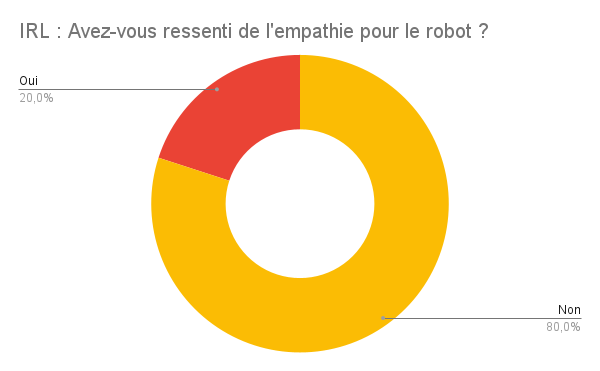
\includegraphics[width=\textwidth]{Datas/IRL _ Avez-vous ressenti de l'empathie pour le robot _.png}
    \captionof{figure}{Physics}
    \end{minipage}%
    \begin{minipage}{.5\textwidth}%
    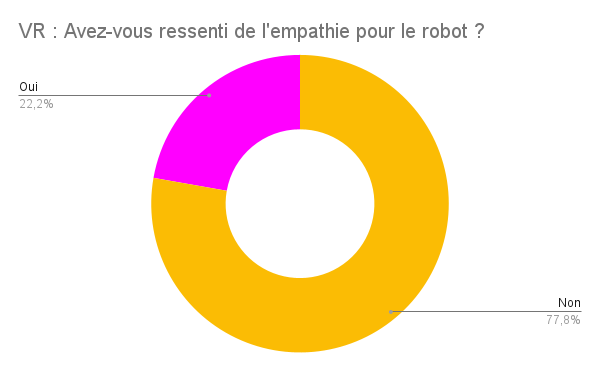
\includegraphics[width=\textwidth]{Datas/VR _ Avez-vous ressenti de l'empathie pour le robot _.png}
    \captionof{figure}{VR}
    \end{minipage}%
    \vspace*{0.5cm}
    
    \subsubsection{Did you get the impression that the robot had a distinct personality?}
    \begin{minipage}{.5\textwidth}%
    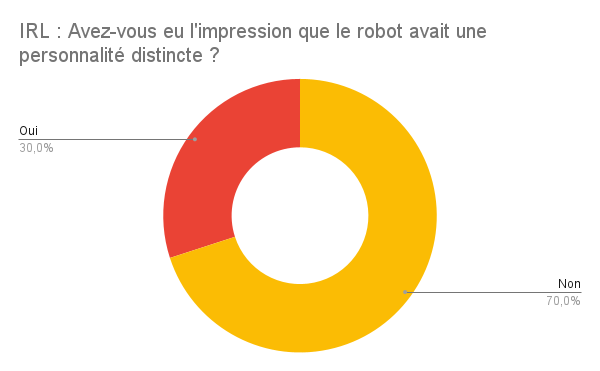
\includegraphics[width=\textwidth]{Datas/IRL_personnalite_distincte.png}
    \captionof{figure}{Physics}
    \end{minipage}%
    \begin{minipage}{.5\textwidth}%
    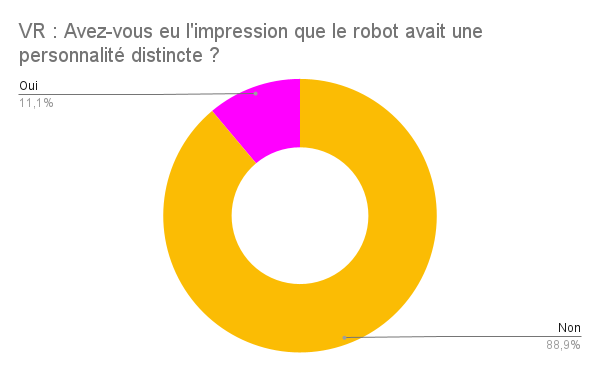
\includegraphics[width=\textwidth]{Datas/VR_personnalite_distincte.png}
    \captionof{figure}{VR}
    \end{minipage}%
    \vspace*{0.5cm}


    \subsubsection{Do you think the robot cheated during the game?}
    \begin{minipage}{.5\textwidth}%
    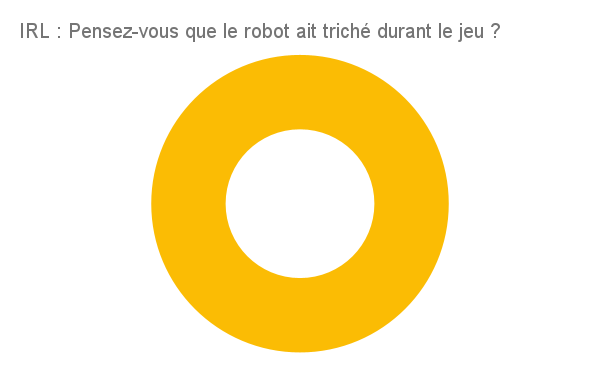
\includegraphics[width=\textwidth]{Datas/IRLtriche.png}
    \captionof{figure}{Physics}
    \end{minipage}%
    \begin{minipage}{.5\textwidth}%
    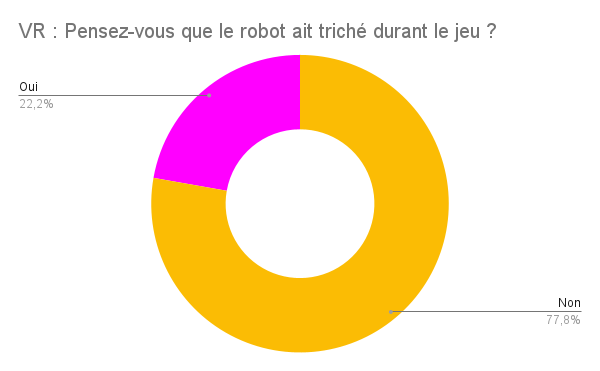
\includegraphics[width=\textwidth]{Datas/VR_triche.png}
    \captionof{figure}{VR}
    \end{minipage}%
    \vspace*{0.5cm}
    
    \subsubsection{How responsive did you find the robot to your answers?}
    \begin{figure}[!h]
    \centering
    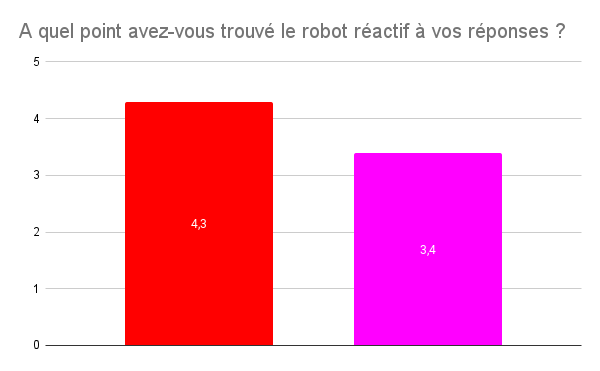
\includegraphics[height=4cm]{Datas/robot_react_reponse.png}
    \caption{Rouge : Physics, Magenta : VR}
    \end{figure}
    \vspace*{0.5cm}

    
    \subsubsection{Did this interaction feel natural to you?}
    \begin{figure}[!h]
    \centering
    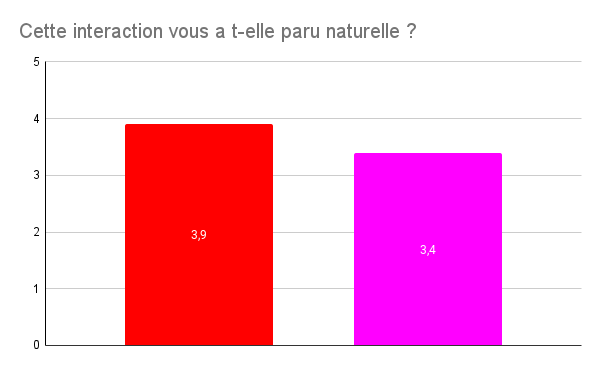
\includegraphics[height=4cm]{Datas/interaction_naturelle.png}
    \caption{Red : Physics, Magenta : VR}
    \end{figure}
    \vspace*{0.5cm}
    \newpage
    
    \subsubsection{How frustrating was the experience?}
    \begin{figure}[!h]
    \centering
    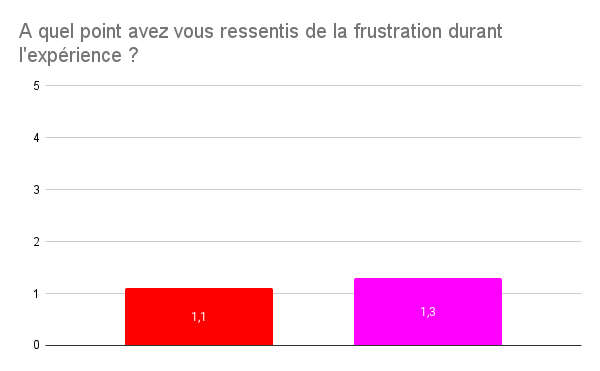
\includegraphics[height=4cm]{Datas/frustration.png}
    \caption{Red : Physics, Magenta : VR}
    \end{figure}
    \vspace*{0.5cm}

    \subsubsection{How did you feel interacting with the robot?}
    \begin{figure}[!h]
    \centering
    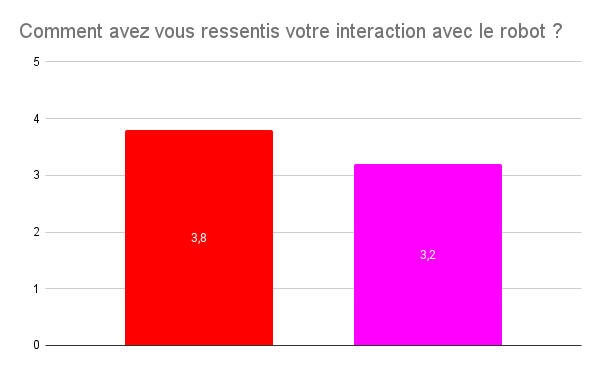
\includegraphics[height=4cm]{Datas/ressenti_interaction.png}
    \caption{Red : Physics, Magenta : VR}
    \end{figure}
    \vspace*{0.5cm}

    \subsubsection{Adult summary :}
Analysis of the data from our experiment revealed some interesting results regarding adults' perceptions of the robot, whether in its physical or VR version. Overall, they showed a relatively low level of empathy towards the robot, whatever its format \textit{(Figure 6.1 / Figure 6.2)}. They also considered that the physical robot possessed a slightly more distinct personality than the VR robot \textit{(Figure 6.3 / Figure 6.4)}.\\
Another notable point is that all the adults felt that the physical robot had not cheated, while some of them thought that the VR robot had adopted deceptive behaviors \textit{(Figure 6.5 / Figure 6.6)}. This divergence of opinion raises interesting questions about the perceived integrity and sincerity of virtual entities compared with those present in the physical world.\\
 They expressed positive impressions of the robots' responsiveness, and the interaction felt natural to them, whether in their physical or VR versions.\textit{(Figure 6.7 / Figure 6.8)} Participants also reported that they didn't feel much frustration throughout the experience \textit{(Figure 6.9)}. This suggests that the robots, whether physical or in VR, were able to provide tailored responses and feedback consistently.\\
\\

    \newpage
\subsection{Children}

    \subsubsection{Did the robot talk like a human?}
    \begin{minipage}{.5\textwidth}%
    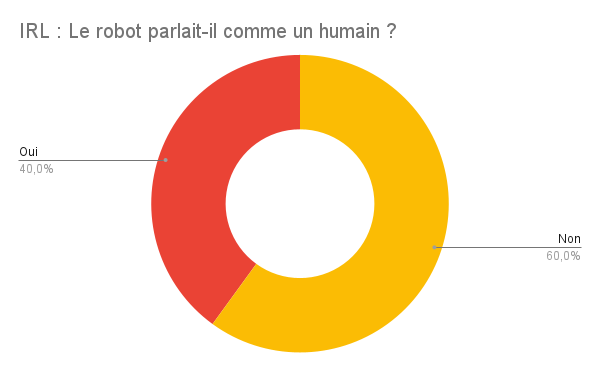
\includegraphics[width=\textwidth]{Datas_childs/IRL _ Le robot parlait-il comme un humain _.png}
    \captionof{figure}{Physics}
    \end{minipage}%
    \begin{minipage}{.5\textwidth}%
    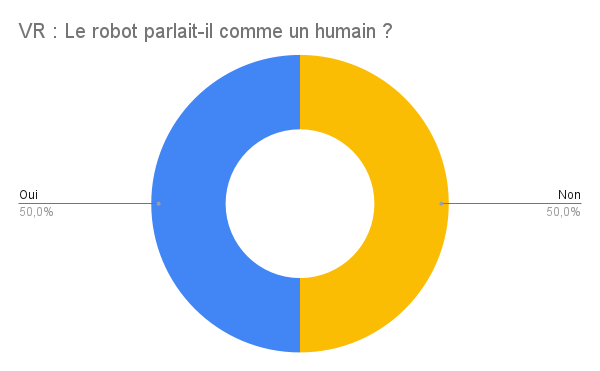
\includegraphics[width=\textwidth]{Datas_childs/VR _ Le robot parlait-il comme un humain _.png}
    \captionof{figure}{VR}
    \end{minipage}%
    \vspace*{0.5cm}

    \subsubsection{Did you feel any sympathy for the robot?}
    \begin{minipage}{.5\textwidth}%
    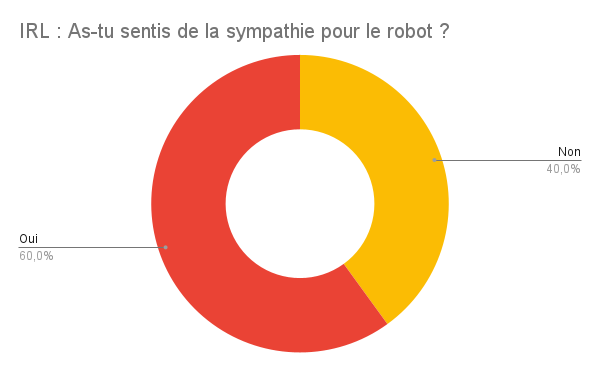
\includegraphics[width=\textwidth]{Datas_childs/IRL _ As-tu sentis de la sympathie pour le robot _.png}
    \captionof{figure}{Physics}
    \end{minipage}%
    \begin{minipage}{.5\textwidth}%
    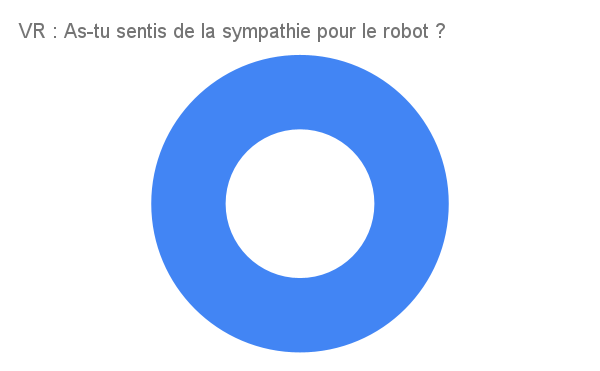
\includegraphics[width=\textwidth]{Datas_childs/VR _ As-tu sentis de la sympathie pour le robot _.png}
    \captionof{figure}{VR}
    \end{minipage}%
    \vspace*{0.5cm}

    \subsubsection{Do you think the robot cheated during the game?}
    \begin{minipage}{.5\textwidth}%
    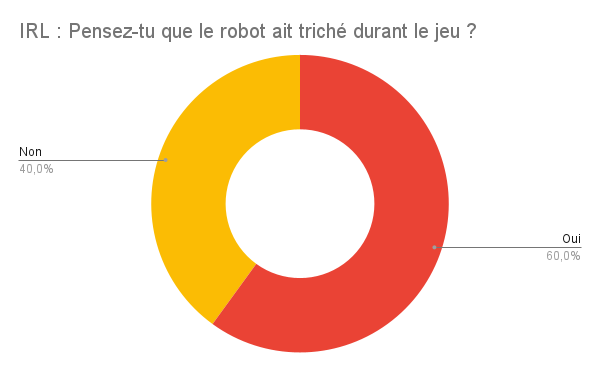
\includegraphics[width=\textwidth]{Datas_childs/IRL_triche_pendant_jeu.png}
    \captionof{figure}{Physics}
    \end{minipage}%
    \begin{minipage}{.5\textwidth}%
    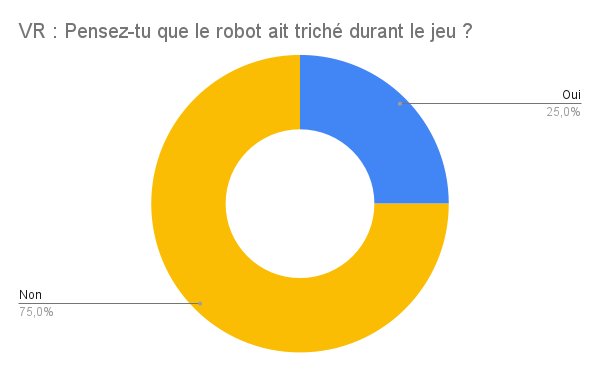
\includegraphics[width=\textwidth]{Datas_childs/VR_triche_pendant_jeu.png}
    \captionof{figure}{VR}
    \end{minipage}%
    \vspace*{0.5cm}
\newpage
    \subsubsection{Was it easy to talk to the robot?}
    \begin{figure}[!h]
    \centering
    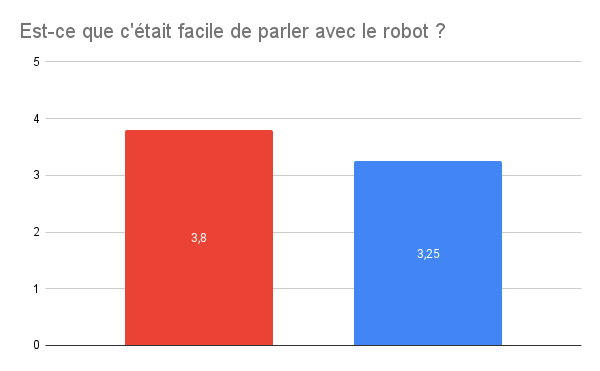
\includegraphics[height=5cm]{Datas_childs/facile_parler.png}
    \caption{Red : Physics, Magenta : VR}
    \end{figure}
    \vspace*{0.5cm}

    \subsubsection{Did the robot react quickly?}
    \begin{figure}[!h]
    \centering
    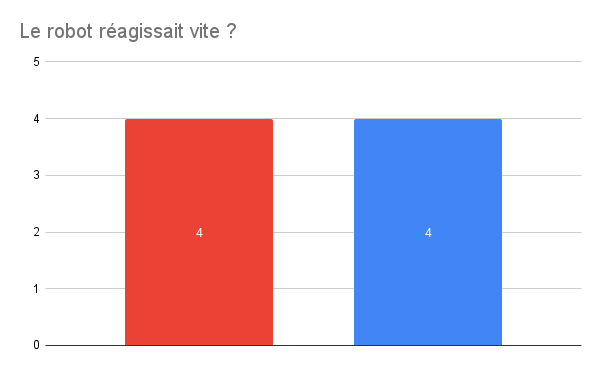
\includegraphics[height=5cm]{Datas_childs/reagit_vite_.png}
    \caption{Red : Physics, Magenta : VR}
    \end{figure}
    
    \vspace*{0.5cm}

    \subsubsection{Did you feel irritated?}
    \begin{figure}[!h]
    \centering
    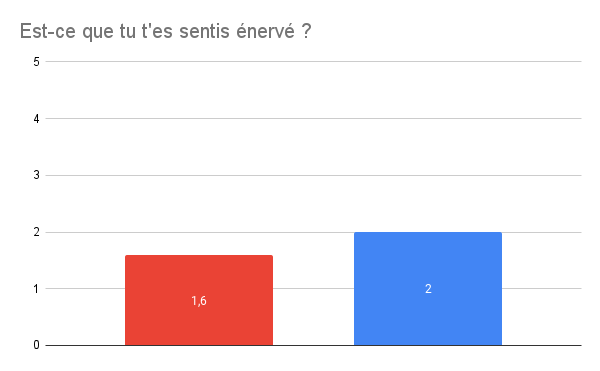
\includegraphics[height=5cm]{Datas_childs/enerve.png}
    \caption{Red : Physics, Magenta : VR}
    \end{figure}
    \vspace*{0.5cm}
    
    \vspace*{0.5cm}

    \subsubsection{Did you feel that the robot was nice or not?}
    \begin{figure}[!h]
    \centering
    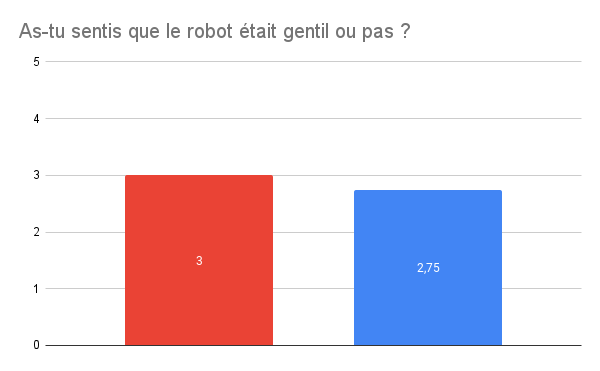
\includegraphics[height=5cm]{Datas_childs/gentil_ou_pas.png}
    \caption{Red : Physics, Magenta : VR}
    \end{figure}
    \vspace*{0.5cm}

\subsubsection{Children :}
During the children's participation in our experiment, interesting observations were made regarding their perception of the robot in virtual reality and in physics. The results show that half the children felt that the VR robot spoke like a human, with a slightly lower proportion for QTrobot \textit{(Figure 6.11 / Figure 6.12)}. It's also interesting to note that all the children felt sympathy towards the VR robot, while slightly more than half felt sympathy towards the physical robot \textit{(Figure 6.13 / Figure 6.14)}. This may suggest that the children were able to engage emotionally with the VR robot, perhaps due to its more abstract representation, whereas the tangible aspect of the physical robot elicited mixed reactions.\\
What's more, only a quarter of the children felt that the VR robot had cheated, while slightly more than half felt this way about the physical robot \textit{(Figure 6.15 / Figure 6.16)}. These results highlight a difference in perception of robot integrity between the two formats. It's possible that the children perceived the VR robot's actions as more controlled by algorithms or scripts, whereas the physical robot seemed to act more spontaneously and authentically.\\
The children found it rather easy to talk to the robot in virtual reality (VR), while it was slightly easier with the physical robot \textit{(Figure 6.17)}. The children also noted that the robots, whether in VR or physics, responded quickly \textit{(Figure 6.18)}. In terms of emotions, the children reported feeling slightly more irritated with the robot in VR, although overall they didn't feel much frustration during the experiment \textit{(Figure 6.19)}. On the other hand, the children gave a rather neutral response as to whether the robot was nice \textit{(Figure 6.20)}.
\newpage
\subsection{Overall summary :}
In conclusion, analysis of the data from our experiment highlights differences in perception and reaction between children and adults towards the robot in virtual reality (VR) and in physical reality. Children showed a greater propensity to perceive the VR robot as speaking like a human, to feel sympathy towards it and to find interaction easy. However, they were slightly more annoyed with the VR robot. On the other hand, adults showed relatively little empathy towards the robot, whether in VR or in physics. What's more, the adults felt that the physical robot had not cheated, while some thought that the VR robot had adopted deceptive behaviors.\\
\\
Both groups, children and adults, appreciated the robot's responsiveness, whether in VR or in physics, as well as the interaction, which was deemed natural. They reported little frustration throughout the experiment, suggesting that the robots were able to provide adapted responses consistently.\\
\\
It should also be noted that the data sample used in our analysis remains relatively small, with the participation of only 20 adults and 9 children. Due to the limited sample size, it is important to consider these results as preliminary observations rather than definitive generalizations. Further studies with larger and more diverse samples would be necessary to confirm and deepen our findings.\\
It's worth pointing out that had we had a larger data sample, we might have considered using machine learning models for further analysis to identify more complex patterns and relationships in the data, which could have provided additional insights into participants' responses, as well as more accurate predictions or classifications.\\
